%% SW design: klassebeskrivelse devkit domain klasser
\newpage

\begin{figure}[htbp] \centering
{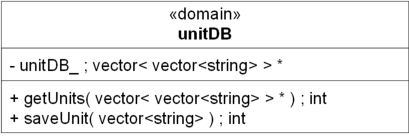
\includegraphics[scale=1.5]{filer/design/Klassediagrammer/sw_unitDB}}
\caption{klassediagram unitDB}
\label{fig:unitDB klassediagram}
\end{figure} 

{\centering
\textbf{unitDB}\par
}
\textbf{Ansvar:} At holde styr på hvor mange enheder der er og deres adresser. \

\verb+int getUnits( & int array, & int size ) +\\
\textbf{Parametre:} Modtager en adresse på et array af integer og en tilhørende referance til at skrive size i.\\
\textbf{Returværdi:} 0 ved succes ellers negativ i overenstemmelse med fejl-listen. \\
\textbf{Beskrivelse:} Metoden skriver sit adresse array over i det array som modtages. Derudover skriver den størrelsen på arrayet over i size så modtageren ved hvor stort arrayet er. (hvor mange golfhuller der er).\\

\verb+int saveUnit( int adresse, int nr = size_ ) +\\
\textbf{Parametre:} Modtager en adresse af typen integer og et index nr. af typen integer. \\
\textbf{Returværdi:} 0 ved succes ellers negativ i overenstemmelse med fejl-listen. \\
\textbf{Beskrivelse:}  Metoden gemmer adressen som modtages på plads nr. Hvis der ikke modtages et index nr, så lægges adressen i array[size] og lægger 1 til size\_. \\


\newpage
\begin{figure}[htbp] \centering
{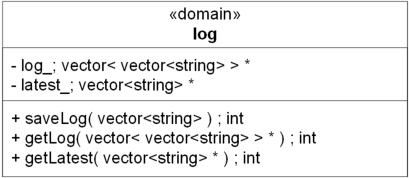
\includegraphics[scale=1.5]{filer/design/Klassediagrammer/sw_log}}
\caption{klassediagram log}
\label{fig:log klassediagram}
\end{figure} 

{\centering
\textbf{log}\par
}
\textbf{Ansvar:} Gemme information loggen til senere brug. \

\verb+int saveLog( vector<string> ) +\\
\textbf{Parametre:} Modtager en vector af typen string. \\
\textbf{Returværdi:} 0 ved succes ellers negativ i overenstemmelse med fejl-listen. \\
\textbf{Beskrivelse:} Modtager log fra Enhed og skriver den over i den samlede log og gemmer den i latest. Loggen skal gemmes i en txt fil som der læses fra under startup. \\

\verb+int getLog( & vector<string> ) + \\
\textbf{Parametre:} Modtager en adresse til en vector af typen string. \\
\textbf{Returværdi:} 0 ved succes ellers negativ i overenstemmelse med fejl-listen. \\
\textbf{Beskrivelse:} Metoden skriver klassens medlems data log over i den adresse som den har modtaget som parameter.\\

\verb+int getLatest( & vector<string> ) +\\
\textbf{Parametre:} Modtager en adresse til en vector af typen string.  \\
\textbf{Returværdi:} 0 ved succes ellers negativ i overenstemmelse med fejl-listen. \\
\textbf{Beskrivelse:} Metoden skriver klassens medlems data latest over i den adresse som den har modtaget som parameter.\\


